\clearpage
\subsection*{PPL de Productie – Maximizare}
\paragraph{}
O fabrică produce două tipuri de pițe congelate, pentru producerea acestor
produse se în calitate de materie primă se folosește aluat, salam, cașcaval și
măsline.Rezerva de materie primă, cantitatea de unități de materie primă
necesara pentru fabricarea unei unități de produs și mărimea venitului obținut
în urma realizării unei unități de produs sunt date in Tabel
~\ref{tab:maximizare}. Este necesar de alcătuit un plan de producție astfel
încât la realizarea ei să obținem venitul maximal.


\paragraph{}
\begin{table}[h]
\centering
\captionsetup{singlelinecheck = false, justification=raggedright}
\caption{Problema de maximizare a venitului}
\label{tab:maximizare}
\begin{center}
\begin{tabular}{|c|c|c|c|}
\hline
	\multirow{2}{3cm}{Tipuri de materie primă} & \multirow{2}{3cm}{Rezerva de materie primă} & \multicolumn{2}{>\centering m{10cm}|}{Cantitatea de materie primă necesară pentru fabricarea unei unități de produs}\\ 
\cline{3-4}
	&& \multicolumn{1}{>\centering m{5cm}|}{Diavola} & \multicolumn{1}{>\centering m{5cm}|}{Atomica}\\ 
\hline
Aluat&2000000&280 &350 \\
Salam&300000&35 &55 \\
Cașcaval&200000&25 &30 \\ 
Măsline&100000&20 &5 \\ 
\hline 
	\multicolumn{2}{|>\centering m{6cm}|}{Venitul de la realizarea unei unități de produs} & 45 & 50\\
\hline
\end{tabular}
\end{center}
\end{table}

\paragraph{Modelul matematic}
Este necesar de gasit valorile nenegative ale variabilelor x și y pentru care funcția Z atinge valoarea maximă.
\begin{gather*}
	Z = 45x + 50y \rightarrow MAX
\end{gather*}
Restricțiile:
\begin{gather*}
	280x + 350y \leq 2000000, \\
	35 x + 55 y \leq 300000, \\
	25 x + 30 y \leq 200000, \\
	20 x + 5 y\leq 100000, \\
	x \geq 0, \; y \geq 0.
\end{gather*}
Rezolvare. Construim tronsonul soluțiilor.
\begin{gather*}
	280x + 350y = 2000000 \; (L1);\\
	35 x + 55 y = 300000 \; (L2); \\
	25 x + 30 y = 200000 \; (L3); \\
	20 x + 5 y= 100000 \; (L4); \\
	x = 0; \; y = 0.
\end{gather*}

\begin{figure}[h]
\begin{center}
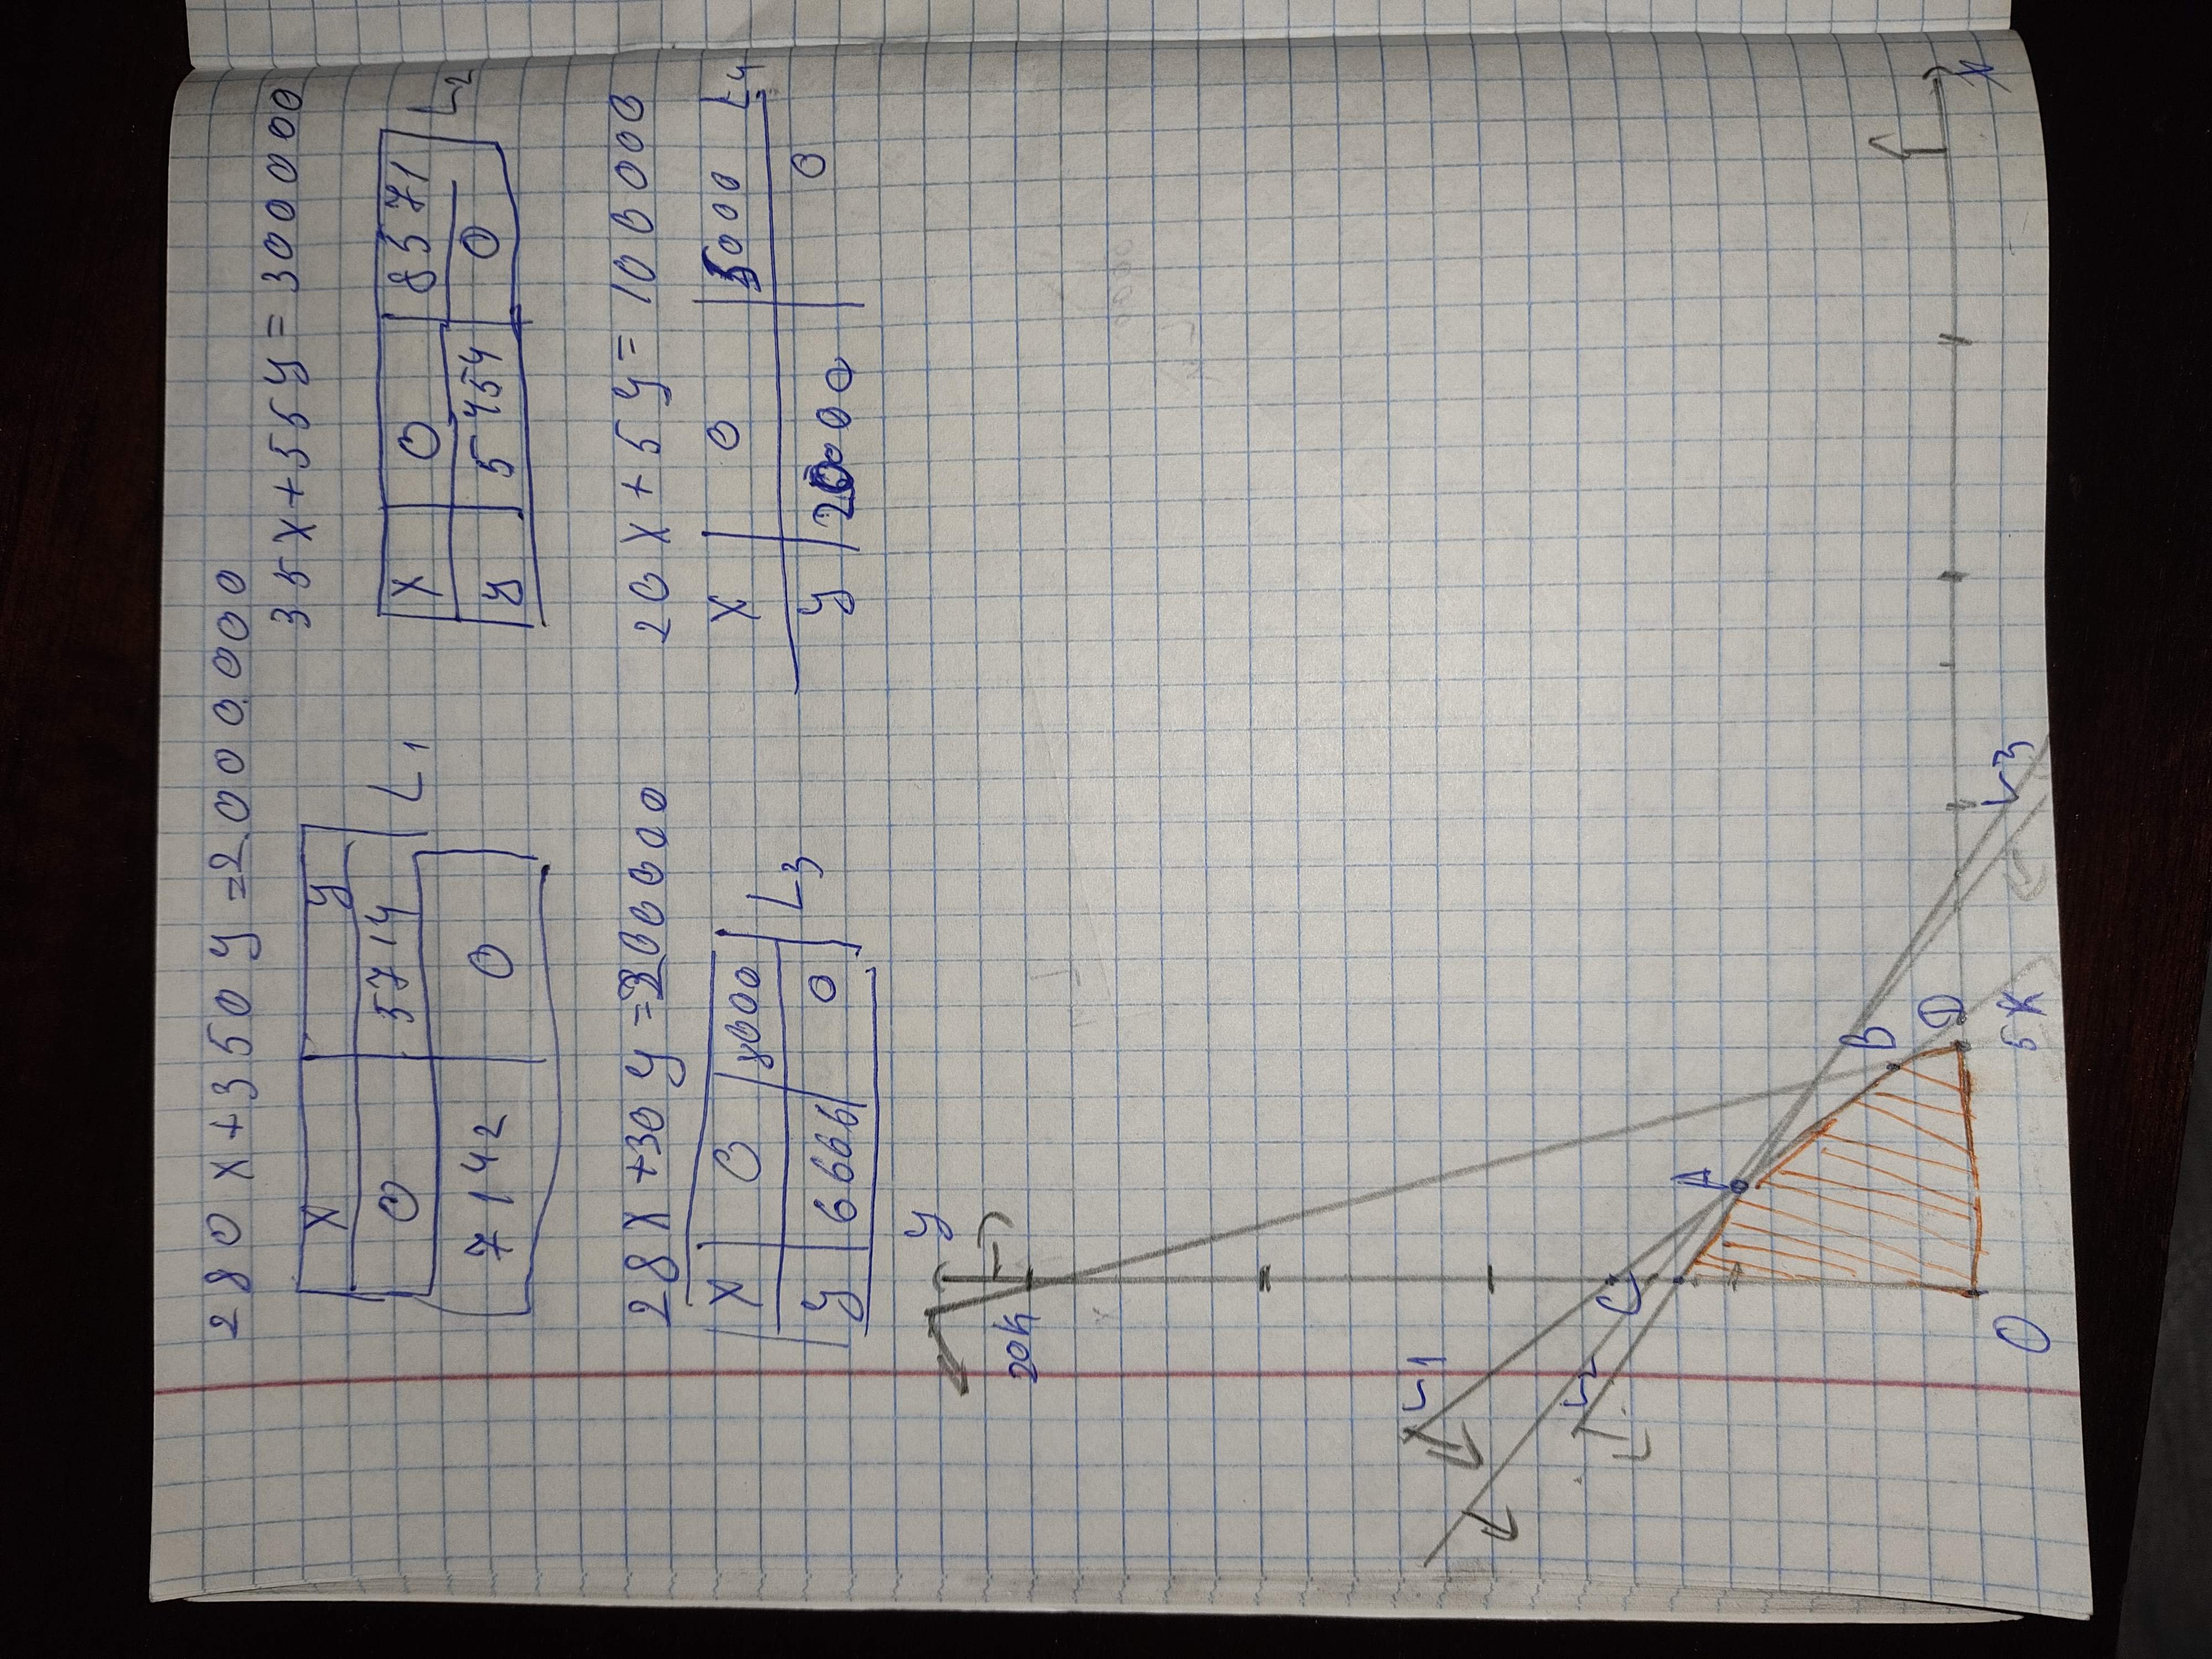
\includegraphics[width=15cm,angle=-90]{maximizare}
\caption{Tronsonul solutiilor admisibile} 
\label{fig:maximizare}
\end{center}
\end{figure}


\paragraph{}
	După cum se vede în Figura ~\ref{fig:maximizare} tronsonul data are 5 vârfuri iar în urma deplasării paralele a dreptei ce corespunde \( 45x + 50y = 0 \) pe vectorul N = (45; 50)\textsuperscript{T}.


\paragraph{}
Tronsonul are următoarele vârfuri: A=(1588,4444), B=(4464,2142), C=(0,5454), \\
D=(5000,0), O=(0,0).
\\
Conform metodei grafice în punctul B profitul este maxim.
\newline
\begin{gather*}
	Z(B) = 45 * 4464 + 50 * 2142 = 307980 \\
	Z(A) = 45 * 1588 + 50 * 4444 = 293666 \\
	Z(C) = 45 * 0 + 50 * 5454 = 272700 \\
	Z(D) = 45 * 5000 + 50 * 0 = 225000 \\
	Z(O) = 0
\end{gather*}


\paragraph{Răspuns }
rezultatul aproximativ este x = 4464; y = 2142. Introducând valorile x și y în funcția liniară, obținem
\begin{equation*}
	Z\textsubscript{MAX}= 45 * 4464 + 50 * 2142 = 307980
\end{equation*}

